\documentclass[10pt]{article}
\usepackage[polish]{babel}
\usepackage[utf8]{inputenc}
\usepackage[T1]{fontenc}
\usepackage{amsmath}
\usepackage{amsfonts}
\usepackage{amssymb}
\usepackage[version=4]{mhchem}
\usepackage{stmaryrd}
\usepackage{graphicx}
\usepackage[export]{adjustbox}
\graphicspath{ {./images/} }

\title{KORESPONDENCYJNY KURS Z MATEMATYKI }

\author{}
\date{}


\begin{document}
\maketitle
\section*{PRACA KONTROLNA nr 1}
październik 2001r

\begin{enumerate}
  \item Dwaj rowerzyści wyruszyli jednocześnie w drogę, jeden z A do B, drugi z B do A i spotkali się po jednej godzinie. Pierwszy z nich przebywał w ciągu godziny o 3 km więcej niż drugi i przyjechał do celu o 27 minut wcześniej niż drugi. Jakie były prędkości obu rowerzystów i jaka jest odległość AB ?
  \item Rozwiązać nierówność:
\end{enumerate}

$$
\sqrt{x^{2}-3}>\frac{2}{x}
$$

\begin{enumerate}
  \setcounter{enumi}{2}
  \item Rysunek przedstawia dach budynku w rzucie poziomym. Każda z płaszczyzn nachy-\\
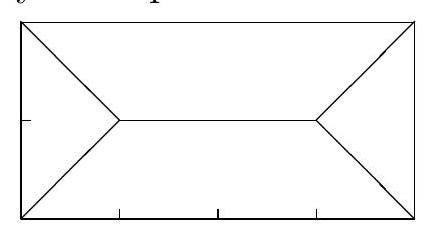
\includegraphics[max width=\textwidth, center]{2024_11_16_494cb7fdc7ec8837e754g-1}\\
lona jest do płaszczyzny poziomej pod kątem $30^{0}$. Długosść dachu wynosi 18 m , a szerokość 9 m . Obliczyć pole powierzchni dachu oraz całkowitą kubaturę strychu w tym budynku.
  \item Pewna firma przeprowadza co kwartał regulację płac dla swoich pracowników rewaloryzując je zgodnie ze wskaźnikiem inflacji, który jest stały i wynosi $1,5 \%$ kwartalnie, oraz doliczając stałą kwotę podwyżki 16 zlp. W styczniu 2001 pan Kowalski otrzymał wynagrodzenie 1600 zlp. Jaką pensję otrzyma w kwietniu 2002? Wyznaczyć wzór ogólny na pensję $w_{n}$ pana Kowalskiego w n-tym kwartale przyjmując, że $w_{1}=1600$ jest płacą w pierwszym kwartale 2001. Obliczyć średnią miesięczną płacę pana Kowalskiego w 2002 roku.
  \item Wyznaczyć funkcję odwrotną do $f(x)=x^{3}, x \in R$. Korzystając z tego wykonać staranny wykres funkcji $h(x)=\sqrt[3]{(|x|-1)}+1$.
  \item Rozwiązać równanie:
\end{enumerate}

$$
\frac{\sin 2 x}{\cos 4 x}=1
$$

\begin{enumerate}
  \setcounter{enumi}{6}
  \item Dany jest trójkąt o wierzchołkach $A(-2,1), \quad B(-1,-6), \quad C(2,5)$. Posługując się rachunkiem wektorowym obliczyć cosinus kąta pomiędzy dwusieczną kąta $A$ i środkową boku $\overline{B C}$. Wykonać rysunek.
  \item Przeprowadzić badanie przebiegu i wykonać wykres funkcji
\end{enumerate}

$$
f(x)=x+\frac{x}{x-1}+\frac{x}{(x-1)^{2}}+\frac{x}{(x-1)^{3}}+\ldots
$$

\section*{PRACA KONTROLNA nr 2}
\begin{enumerate}
  \item Cena 1 l paliwa została zmniejszona o $15 \%$. Po dwóch tygodniach dokonano kolejnej zmiany ceny paliwa zwiększając ją o $15 \%$. O ile procent końcowa cena paliwa różni się od początkowej?
  \item Wyznaczyć i narysować zbiór złożony z punktów $(x, y)$ płaszczyzny spełniających warunek
\end{enumerate}

$$
x^{2}+y^{2}=8|x|+6|y|
$$

\begin{enumerate}
  \setcounter{enumi}{2}
  \item Wysokość ostrosłupa trójkątnego prawidłowego wynosi $h$, a kąt między wysokościami ścian bocznych jest równy $2 \alpha$. Obliczyć pole powierzchni bocznej tego ostrosłupa. Sporządzić odpowiednie rysunki.
  \item Z arkusza blachy w kształcie równoległoboku o bokach 30 cm i 60 cm i kącie ostrym $60^{0}$ należy odciąć dwa przeciwległe trójkątne naroża tak, aby powstał romb o możliwie największym polu. Określić przez który punkt dłuższego boku należy przeprowadzić cięcie oraz obliczyć kąt ostry otrzymanego rombu zaokrąglając wynik do jednej minuty kątowej.
  \item Rozwiązać równanie
\end{enumerate}

$$
2^{\log _{\sqrt{2}} x}=(\sqrt{2})^{\log _{x} 2}
$$

\begin{enumerate}
  \setcounter{enumi}{5}
  \item Wyznaczyć dziedzinę i zbiór wartości funkcji
\end{enumerate}

$$
f(x)=\frac{4}{\sin x+2 \cos x+3} .
$$

\begin{enumerate}
  \setcounter{enumi}{6}
  \item Znaleźć wszystkie wartości parametru $p$, dla których równanie
\end{enumerate}

$$
p x^{4}-4 x^{2}+p+1=0
$$

ma dwa różne rozwiązania.\\
8. Wyznaczyć tangens kąta, pod którym styczna do wykresu funkcji $f(x)=\frac{8}{x^{2}+3} \mathrm{w}$ punkcie $A\left(3, \frac{2}{3}\right)$ przecina wykres tej funkcji.

\section*{PRACA KONTROLNA nr 3}
grudzień 2001r

\begin{enumerate}
  \item Dla jakich wartości $\sin x$ liczby $\sin x, \cos x, \sin 2 x$ (w podanym porządku) są kolejnymi wyrazami ciągu geometrycznego. Wyznaczyć czwarte wyrazy tych ciągów.
  \item W pewnych zawodach sportowych startuje 16 drużyn. W eliminacjach są one losowo dzielone na 4 grupy po 4 drużyny każda grupa. Obliczyć prawdopodobieństwo tego, że trzy zwycięskie drużyny z poprzednich zawodów znajdą się każda w innej grupie.
  \item Nie wykonując dzielenia udowodnić, że wielomian $\left(x^{2}+x+1\right)^{3}-x^{6}-x^{3}-1$ dzieli się bez reszty przez trójmian $(x+1)^{2}$.
  \item Wyznaczyć równanie okręgu o promieniu $r$ stycznego do paraboli $y=x^{2} \mathrm{w}$ dwóch punktach. Dla jakiego $r$ zadanie ma rozwiązanie? Sporządzić rysunek przyjmując $r=3 / 2$.
  \item Stosując zasadę indukcji matematycznej udowodnić prawdziwość wzoru
\end{enumerate}

$$
\binom{2}{2}-\binom{3}{2}+\binom{4}{2}-\binom{5}{2}+\ldots+\binom{2 n}{2}=n^{2}, \quad n \geqslant 1
$$

\begin{enumerate}
  \setcounter{enumi}{5}
  \item Rozwiązać nierówność:
\end{enumerate}

$$
\log _{x}\left(1-6 x^{2}\right) \geqslant 1
$$

\begin{enumerate}
  \setcounter{enumi}{6}
  \item Środek $S$ okręgu wpisanego w trapez $A B C D$ jest odległy od wierzchołka $B$ o $S B=$ d, a krótsze ramię $\overline{B C}$ ma długość $B C=\mathrm{c}$. Punkt styczności okręgu z krótszą podstawą dzieli ją w stosunku 1:2. Obliczyć pole tego trapezu. Wykonać rysunek dla $\mathrm{c}=5 \mathrm{i} d=4$.
  \item Wszystkie ściany równoległościanu są rombami o boku $a$ i kącie ostrym $\beta$. Obliczyć objętość tego równoległościanu. Sporządzić rysunek. Obliczenia poprzeć stosownym dowodem.
\end{enumerate}

\section*{PRACA KONTROLNA nr 4}
styczeń 2002r

\begin{enumerate}
  \item Obliczyć granicę ciągu o wyrazie ogólnym
\end{enumerate}

$$
a_{n}=\frac{2^{n}+2^{n+1}+\ldots+2^{2 n}}{2^{2}+2^{4}+\ldots+2^{2 n}}
$$

\begin{enumerate}
  \setcounter{enumi}{1}
  \item Wyznaczyć równanie prostej prostopadłej do danej $2 x+3 y+3=0$ i leżącej w równej odległości od dwóch danych punktów $A(-1,1)$ i $B(3,3)$. Sporządzić rysunek.
  \item Tworząca stożka ma długość $l$ i widać ją ze środka kuli wpisanej w ten stożek pod kątem $\alpha$. Obliczyć objętość i kąt rozwarcia stożka. Określić dziedzinę kąta $\alpha$.
  \item Bolek kupił jeden długopis i $k$ zeszytów i zapłacił $k$ zł i 50 gr, a Lolek kupił $k$ długopisów i 4 zeszyty i zapłacił $2,5 k$ zł. Wyznaczyć cenę długopisu i zeszytu w zależności od parametru $k$. Znaleźć wszystkie możliwe wartości tych cen wiedząc, że zeszyt kosztuje nie mniej niż 50 gr, długopis jest droższy od zeszytu, a ceny obydwu artykułów wyrażają się w pełnych złotych i dziesiątkach groszy.
  \item Rozwiązać nierówność:
\end{enumerate}

$$
\operatorname{tg}^{3} x \geqslant \sin 2 x
$$

\begin{enumerate}
  \setcounter{enumi}{5}
  \item Żarówki są sprzedawane w opakowaniach po 6 sztuk. Prawdopodobieństwo, że pojedyncza żarówka jest sprawna wynosi $\frac{2}{3}$. Jakie jest prawdopodobieństwo tego, że w jednym opakowaniu znajdą się co najmniej 4 sprawne żarówki. O ile wzrośnie to prawdopodobieństwo, jeśli jedna, wylosowana z opakowania żarówka okazała się sprawna.
  \item Prosta styczna w punkcie $P$ do okręgu o promieniu 2 i półprosta wychodząca ze środka okręgu mająca z okręgiem punkt wspólny $S$ przecinają się w punkcie $A$ pod kątem $60^{\circ}$. Znaleźć promień okręgu stycznego do odcinków $A P, A S$ i łuku $P S$. Wykonać odpowiedni rysunek.
  \item W ostrosłupie prawidłowym, którego podstawą jest kwadrat, pole każdej z pięciu ścian wynosi 1. Ostrosłup ten ścięto płaszczyzną równoległą do podstawy tak, aby uzyskać maksymalny stosunek objętości do pola powierzchni całkowitej. Obliczyć pole powierzchni całkowitej otrzymanego ostrosłupa ściętego. Rozwiązanie zilustrować rysunkiem.
\end{enumerate}

\section*{PRACA KONTROLNA nr 5}
luty 2002r

\begin{enumerate}
  \item W czworokącie $A B C D$ dane są wktory $\overrightarrow{A B}=(2,-1), \overrightarrow{B C}=(3,3), \overrightarrow{C D}=(-4,1)$. Punkty $K$ i $M$ są środkami boków $\overline{C D}$ oraz $\overline{A D}$. Posługując się rachunkiem wektorowym obliczyć pole trójkąta $K M B$. Wykonać rysunek.
  \item Krawędzie oraz przekątna prostopadłościanu tworzą cztery kolejne wyrazy ciągu arytmetycznego. Wyznaczyć sumę długości wszystkich krawędzi tego prostopadłościanu, jeśli przekątna ma długość 7 cm .
  \item Na płaszczyźnie Oxy dane są zbiory:
\end{enumerate}

$$
A=\left\{(x, y): y \leqslant \sqrt{5 x-x^{2}}\right\}, \quad B_{s}=\{(x, y): 3 x+4 y=s\}
$$

Dla jakich wartości parametru $s$ zbiór $A \cap B_{s}$ nie jest pusty? Sporządzić rysunek.\\
4. Działka gruntu ma kształt trapezu o bokach $20 \mathrm{~m}, 30 \mathrm{~m}, 40 \mathrm{~m}$ i 60 m . Właściciel działki twierdzi, że pole jego działki wynosi ponad 11 arów. Czy właściciel ma rację? Jeśli tak, to narysować plan działki w skali 1:1000 i podać dokładną wartość jej pola.\\
5. Dane jest równanie kwadratowe z parametrem $m$ :

$$
(m+2) x^{2}+4 \sqrt{m} x+(m-3)=0
$$

Dla jakiej wartości parametru $m$ kwadrat różnicy pierwiastków rzeczywistych tego równania jest największy. Podać tę największą wartość.\\
6. Stosując zasadę indukcji matematycznej udowodnić, że dla każdego $n \geqslant 2$ liczba $2^{2^{n}}-6$ jest podzielna przez 10 .\\
7. Rozwiązać układ równań

$$
\left\{\begin{array}{l}
\operatorname{tg} x+\operatorname{tg} y=4 \\
\cos (x+y)+\cos (x-y)=\frac{1}{2}
\end{array} \quad \text { dla } x, y \in[-\pi, \pi]\right.
$$

\begin{enumerate}
  \setcounter{enumi}{7}
  \item Równoramienny trójkąt prostokątny $A B C$ zgięto wzdłuż środkowej $\overline{C D}$ wychodzącej z wierzchołka kąta prostego $C$ tak, aby obie połowy tego trójkąta utworzyły kąt $60^{\circ}$. Obliczyć sinusy wszystkich kątów dwuściennych otrzymanego czworościanu $A B C D$. Wykonać odpowiednie rysunki i uzasadnić obliczenia.
\end{enumerate}

\section*{PRACA KONTROLNA nr 6}
marzec 2002r

\begin{enumerate}
  \item Wyznaczyć wszystkie wartości parametru rzeczywistego $m$, dla których osią symetrii wykresu funkcji $p(x)=\left(m^{2}-2 m\right) x^{2}-(2 m-4) x+3$ jest prosta $x=m$. Wykonać rysunek.
  \item Z kuli o środku w zerze i promieniu $R$ wycięto ósmą jej część trzema płaszczyznami układu współrzędnych. W tak otrzymaną bryłę wpisano kulę. Obliczyć stosunek pola powierzchni tej kuli do pola powierzchni bryły.
  \item W trzech pustych urnach K, L, M rozmieszczamy losowo 4 różne kule. Obliczyć prawdopodobieństwo tego, że żadna z urn K i L nie pozostanie pusta.
  \item Dane są punkty $A(2,6), B(-2,6)$ i $C(0,0)$, Wyznaczyć równanie linii zawierającej wszystkie punkty trójkąta $A B C$, dla których suma kwadratów ich odległości od trzech boków jest stała i wynosi 9. Sporządzić rysunek.
  \item Sporządzić dokładny wykres i napisać równania asymptot funkcji
\end{enumerate}

$$
f(x)=\frac{(x+1)^{2}-1}{x|x-1|}
$$

nie przeprowadzając badania jej przebiegu.\\
6. Rozwiązać nierówność:

$$
|x|^{2 x-1} \leqslant \frac{1}{x^{2}}
$$

\begin{enumerate}
  \setcounter{enumi}{6}
  \item Styczna do wykresu funkcji $f(x)=\sqrt{3+x}+\sqrt{3-x}$ w punkcie $A\left(x_{0}, f\left(x_{0}\right)\right)$ przecina oś x w punkcie $P$, a oś y w punkcie $Q$ tak, że $O P=O Q$. Wyznaczyć $x_{0}$.
  \item Trójkąt równoboczny o boku $a$ przecięto prostą $l$ na dwie figury, których stosunek pól jest równy 1:5. Prosta ta przecina bok $\overline{A C}$ w punkcie $D$ pod kątem $15^{0}$, a bok $\overline{A B}$ w punkcie $E$. Wykazać, że $A D+A E=a$.
\end{enumerate}

\section*{PRACA KONTROLNA nr 7}
kwiecień 2002r

\begin{enumerate}
  \item Sześcian o krawędzi długości 3 cm ma taką samą objętość jak dwa sześciany, których suma długości obydwu krawędzi wynosi 4 cm . O ile $\mathrm{cm}^{2}$ pole powierzchni dużego sześcianu jest mniejsze od sumy pól powierzchni dwóch mniejszych sześcianów.
  \item Obliczyć tangens kąta utworzonego przez przekątne czworokąta o wierzchołkach $\mathbf{A}(\mathbf{1}, \mathbf{1}), \mathrm{B}(\mathbf{2}, \mathbf{0}), \mathrm{C}(\mathbf{2}, 4), \mathrm{D}(\mathbf{0}, \mathbf{6})$. Rozwiązanie zilustrować rysunkiem.
  \item W trójkąt prostokątny wpisano okrąg, a w okrąg ten wpisano podobny trójkąt prostokątny. Wyznaczyć cosinusy kątów ostrych trójkąta, jeśli wiadomo, że stosunek pól obu trójkątów wynosi 9.
  \item Wykazać, że ciąg $a_{n}=\sqrt{n(n+1)}-n$ jest rosnący. Obliczyć jego granicę.
  \item Rozwiązać nierówność:
\end{enumerate}

$$
2 \cos ^{2} \frac{x}{4}>1
$$

\begin{enumerate}
  \setcounter{enumi}{5}
  \item Rozwiązać równanie
\end{enumerate}

$$
\log _{2}(1-x)+\log _{4}(x+4)=\log _{4}\left(x^{3}-x^{2}-3 x+5\right)+\frac{1}{2}
$$

nie wyznaczając dziedziny w sposób jawny.\\
7. W kulę o promieniu $R$ wpisano stożek o największej objętości. Wyznaczyć promień podstawy $r$ i wysokość $h$ tego stożka. Sporządzić rysunek.\\
8. Znaleźć równania wszystkich prostych, które są styczne jednocześnie do krzywych

$$
y=-x^{2}, \quad y=x^{2}-8 x+18
$$

Sporządzić rysunek.


\end{document}